\documentclass[utf8]{article}
\usepackage{import}
\usepackage{WritingToolsByAcer}

% \excludeversion{WritingMaterials}
% \excludeversion{backup}

\usepackage{chngcntr}
\counterwithout{figure}{section}

%% ================================== acronym ================================= %
\usepackage{acronym}
\newacro{ntic}[NTIC]{non-trivial informational closure}
\newacro{ic}{informational closure}
\newacro{cg}{coarse-grain}
\newacro{cging}{coarse-graining}
\newacro{cged}{coarse-grained}
\newacro{ncg}{neural coarse-graining}
\newacro{OurTheory}[ICT]{Information Closure Theory of Consciousness}


% ============================================================================ %
%                                     Title                                    %
% ============================================================================ %
\title{Information Closure Theory of Consciousness}



% ============================================================================ %
%                                    Authors                                   %
% ============================================================================ %
\author[]{Acer Y.C. Chang\thanks{acercyc@araya.org}}
\author[]{Martin Biehl\thanks{martin@araya.org}}
\author[]{Yen Yu\thanks{yen.yu@araya.org}}
\author[]{Ryota Kanai\thanks{kanair@araya.org }}
\affil[]{ARAYA, Inc., Tokyo, Japan}



% ============================================================================ %
%                                     Body                                     %
% ============================================================================ %
\begin{document}
    \linenumbers
	\maketitle
	\tableofcontents


	\begin{abstract}
		Neural systems process information through different levels of organisation in a hierarchical manner. Information at lower levels is finer-grained and can be coarse-grained for higher level computation. However, one is aware of information processed only at specific levels. Theorists have addressed this issue. For example, the intermediate level theory of consciousness suggests that the intermediate level seems to be privileged with respect to consciousness. It is true that we do not experience information processed by individual neurons which is always highly stochastic noisy. In addition, we have no conscious experience from interpersonal activities despite massive interactions among individuals. Instead, neurophysiological evidence has been showing that conscious experience tends to co-vary with information encoded in coarse-grained neural states such as neural population codes. We argue that the content of consciousness is determined by neural variables that obey informational closure and that other brain processes remain unconscious. Out theory based on concise assumptions and propose quantitative definitions using information theorem for both conscious content and conscious level.
		
	\end{abstract}


	\section*{Keywords:}
	Keywords: consciousness, informational closure, neural coarse-graining, level of analysis


% ============================================================================ %
    \newpage
    \section*{Not decided terminology}
        \begin{ants}
            @ information * in the NTIC process
            @ Full and short name of this theory
            @ core "?" (entity) for conscious content 
            @ our theory? framework? proposal? 
            @ system? process?
            @ variable? node? element? member?
            @ TODO:
                @@ Change coarse-graining function to "aggregation function"
            @ Decided
                @@ "form" NTIC
            @ Replacement
                @ correlate -> ?
                @ information processing -> ?
                @ achieve -> form
        \end{ants}

% ============================================================================ %
    \newpage
    \section*{Discussion points}
        \begin{ants}
            @ I can understand that an NTIC process must be coarse-graining of the "full process" (Environment + NTIC or we say {E, Y}). But I am still thinking is this the same as my original idea that variables forming the NTIC process are coarse-grained from microscopic variables? This is very critical to how we present this paper. 
            
        \end{ants}    
    
% ============================================================================ %
%                                     Start                                    %
% ============================================================================ %

    \newpage
	\section{Introduction}

		%% Story about a cell
		Imagine you are a neuron in Alice's brain. Your daily work is to collect neurotransmitters through dendrites from other neurons, accumulate membrane potential, and finally send signals to other neurons through action potentials along axons. However, you have no idea that you are one of the neurons in Alice's supplementary motor area and involved in many motor control processes for Alice's action, for example, grabbing a cup. You are ignorant of intentions, goals, and motor plans that Alice has at every moment even though you are part of the physiological substrate responsible for all those actions.
		A similar story also happens to Alice's conscious mind. To grab a cup, for example, Alice is conscious of her intention and visuosensory experience of this action. However, her conscious experience does not reflect the dynamic of your membrane potential or the action potentials you send to other neurons every second. That is, not all information you have is available to Alice's conscious mind.

		%% scale
		
		It seems to be true that we are not consciously accessing information processed at every scale in the neural system. There are both more microscopic and more macroscopic levels than the level corresponding to the conscious contents. On the one hand, dynamics of individual neurons are stochastic \citep{Goldwyn2011, White2000}. However, what we are aware of in our conscious mind shows astonishing stability and robustness against the ubiquitous noise in the neural system \citep{mathis1995computational}. In addition, some parts of the neural system contribute very little to conscious experience (the cerebellum for example \citep{lemon2010life}), also suggesting that conscious contents do not have one-to-one mapping to the entire state of the neural system. On the other hand, human conscious experience is more detailed than just a simple (e.g. binary) process can represent, suggesting that the state space of conscious experience is much larger than what a single overly coarse-grained binary variable can represent. These facts suggest that conscious processes are scale dependent. We refer to this notion as \textbf{the scale problem of consciousness} (Fig.~\ref{fig:scaleproblem}).

		%% our argument
		In this article, we propose a new information-based theory of consciousness, called \ac{OurTheory}. We argue that every process with a high degree of not-trivial information closure (NTIC) has consciousness. This means that the state of such a process corresponds one-to-one to conscious content.\footnote{In the following IC stands for "informational closure" or "informationally closed" and NTIC stands for "non-trivial informational closure" or "non-trivially informationally closed".}. We further postulate that the \textit{level} of consciousness corresponds to the degree of NTIC. (for the level versus content of consciousness see \cite{laureys2005neural, overgaard2010neural}).
		
		In the following, we first introduce non-trivial informational closure and its importance to information processing for human scale agents (Sec.\ref{sec:Non-trivial informational closure}). We next argue that through coarse-graining the neural system can form a high degree of NTIC at a specific coarse-grained level (Sec.\ref{sec:Neural coarse-graining}). In the Sec.\ref{sec:OurTheory}, we propose our theory: \acf{OurTheory}. We also illustrate how \ac{OurTheory} can parsimoniously explain empirical findings from previous consciousness studies (Sec.\ref{sec:Conscious versus Unconscious Processing}) and reconcile several current major theories of consciousness (Sec.\ref{sec:Comparison with other theories}). Finally, we discuss the current theoretical and empirical limitations of \ac{OurTheory} and propose the implications from this theory to the current consciousness science (Sec.\ref{sec:Limitation and Future work}). 


		\begin{figure}[H]
		    \centering
			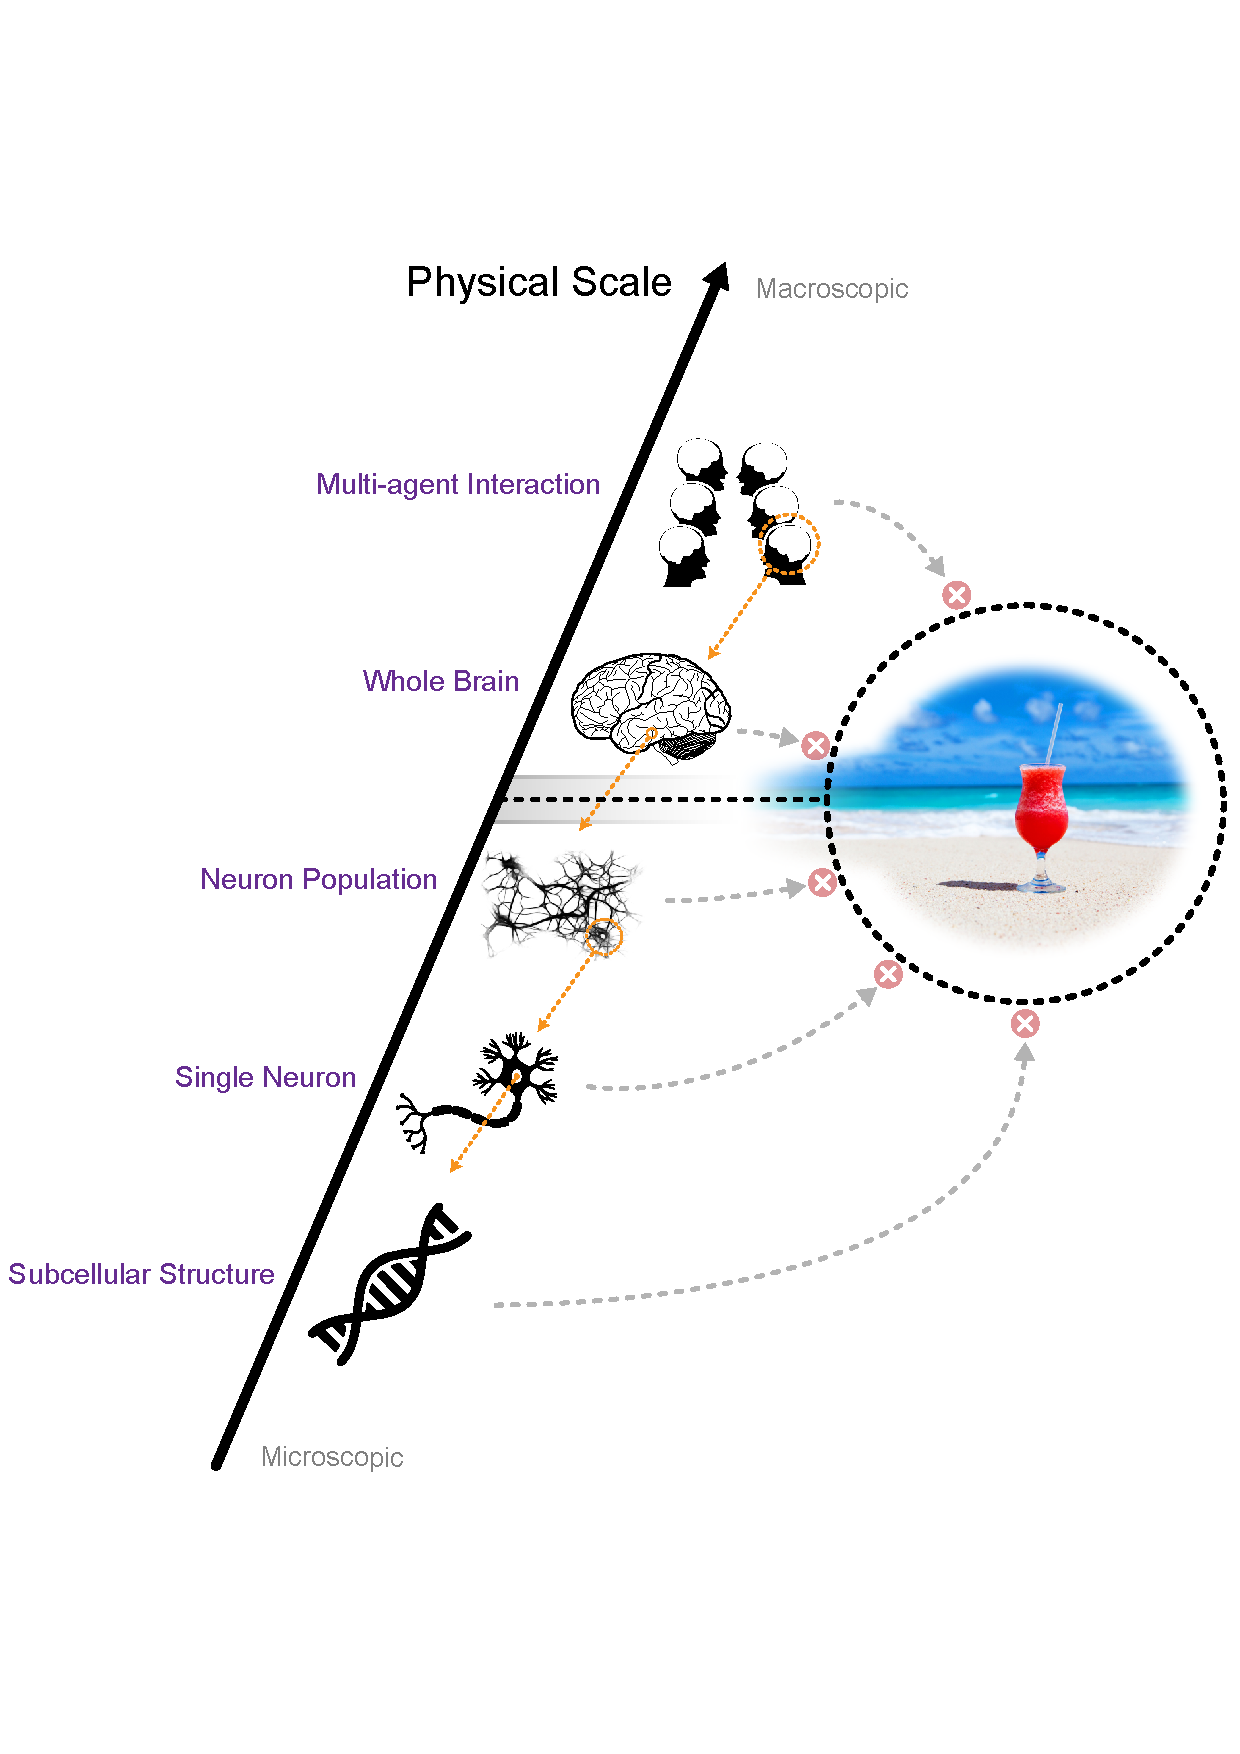
\includegraphics[width=\textwidth]{WritingMaterials/Fig_ScaleProblemOfConsciousness/ScaleProblemOfConsciousness.pdf}
			\caption{The scale problem of consciousness: Human conscious experience does not reflect information processed at every scale. Only information at a certain coarse-grained scale in the neural system is conscious.}
			\label{fig:scaleproblem}
	   	\end{figure}


% ============================================================================ %
%                       Non-trivial informational closure                      %
% ============================================================================ %
	\section{Non-trivial informational closure} \label{sec:Non-trivial informational closure}
		The notion of non-trivial informational closure (NTIC) is introduced by \cite{BERTSCHINGER.2006}. The concept of closure is closely related to system identification in systems theory. One can distinguish a system from its environment by computing the closeness of the system \citep{maturana1991autopoiesis, rosen1991life, pattee2012evolving, luhmann1995probleme}. The closure can be further quantified by information theory.



		% Definition of informational closure
			\noindent
			Consider two processes, the environment process $(E_t)_{t \in \mathbb{N}}$ and the system's process $(Y_t)_{t \in \mathbb{N}}$ and let their interaction be described by the Bayesian network in Fig.~\ref{fig:SystemAndEnv}. Then, information flow $J_{t}$ from the environment $E$ to a system $S$ at time $t$ can be defined as the conditional mutual information $I$ between the current environment state $E_{t}$  and the future system state $Y_{t+1}$ given the current system state $Y_{t}$

				\begin{equation}
    				\label{eq:InformationFlow}
    				\left.\begin{array}
    				{rl}{J_{t}(E \rightarrow Y )} & {:= I(Y_{t+1};E_{t}|Y_{t})} \\
    				%{ } & { \ = H(Y_{t+1}|Y_{t})-H(Y_{t+1}|Y_{t},E_{t})} \\
    				%{ } & { \ = H(E_{t}|Y_{t})-H(Y_{t}|Y_{t},Y_{t+1})} \\
    				%{ } & { \ = H(E_{t}|Y_{t})-H(E_{t}|Y_{t},Y_{t+1})}\\
    				{ } & { \ = I(Y_{t+1};E_{t}) - (I(Y_{t+1};Y_{t})-I(Y_{t+1};Y_{t}|E_{t}))}
    				\end{array}\right.
				\end{equation}

            
				\begin{figure}
					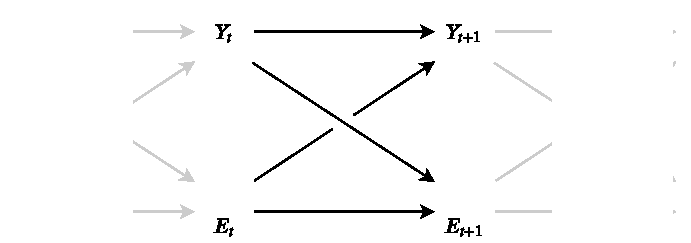
\includegraphics[width=\textwidth]{WritingMaterials/Fig_SystemAndEnv/SystemAndEnv_2.pdf}
					\caption{The dependencies between a system and its environment.} % Figure adapted from \cite{BERTSCHINGER.2006}
					\label{fig:SystemAndEnv}
				\end{figure}
				\todo{Modify this figure}


			\noindent
			\cite{BERTSCHINGER.2006} defines that a system is informationally closed when information flow from the environment to the system is zero.

				\begin{equation}
				J_{t}(E \rightarrow Y )=0
				\label{eq:informationflow2}
				\end{equation}


			% ------------------------------- trivial case ------------------------------- %
			\noindent
			Information closure (minimising $J_t$) is trivial if the environment and the system are entirely independent of each other.

				\begin{equation}
				\begin{aligned}
				{I(Y_{t+1};E_{t})=0}&&{\Rightarrow}&&{J_{t}(E \rightarrow Y )=0}
				\end{aligned}
				\end{equation}


			% -------------------------------- non-trivial ------------------------------- %
			\noindent
			However, informational closure can be formed non-trivially. In the non-trivial case, even though a system contains (or encodes) information about the environmental dynamics, the system can still be informationally closed. In such cases, the mutual information between the current states of the environment and the future state of the system is larger than zero. %\footnote{Here we assume that that the environment contains more information than the system, i.e. $H(E|S)>0$ and $E\neq S$}. 

				\begin{equation}
				I(Y_{t+1};E_{t}) > 0
				\end{equation}

			\noindent
			This also implies
				\begin{equation}
					I(Y_{t+1};Y_{t})-I(Y_{t+1};Y_{t}|E_{t}) > 0
				\end{equation}



			\noindent
			And, non-trivial informational closure can be defined as
				\begin{equation}
				\label{eq:NTIC}
    				\left.\begin{array}
    				{rl}{NTIC} & {:=I(Y_{t+1};Y_{t})-I(Y_{t+1};Y_{t}|E_{t})}
    				\end{array} \right.
				\end{equation}
				
				
			\noindent
            The definition can also be re-arranged as 
				\begin{equation}
				\label{eq:NTIC2}
    				\left.\begin{array}
    				{rl}{\qquad} & {\ =I(Y_{t+1};E_{t})-I(Y_{t+1};E_{t}|Y_{t})}
    				\end{array} \right.
				\end{equation}				

			\noindent
			Hence, maximising NTIC amounts to
				\begin{equation}
    				\label{eq:nticObjective}
    				\begin{aligned}
    				& \text{maximising} & { } & I(Y_{t+1};Y_{t}) & { } & \text{and} \\
    				& \text{minimising} & { } & I(Y_{t+1};Y_{t}|E_{t}) & { }
    				\end{aligned}
				\end{equation}
				
			One can also maximise NTIC by 
				\begin{equation}
    				\label{eq:nticObjective2}
    				\begin{aligned}
    				& \text{maximising} & { } & I(Y_{t+1};E_{t}) & { } & \text{and} \\
    				& \text{minimising} & { } & I(Y_{t+1};E_{t}|Y_{t}) & { }
    				\end{aligned}
				\end{equation}			

			\noindent
			This implies the system contains in itself all the information about its own future and the self-predictive information is gained from the information about the environment. Therefore, to form NTIC, the system can internalise and synchronise the dynamics of the environment, i.e. modelling the environment. Furthermore, having high degrees of NTIC entails having high predictive power about the environment. This gives biological agents a great functional and evolutionary advantage. 
			
			% Practically, \cite{guttenberg2016neural} proposed that NTIC can be formed by maximising the predictive power about the environment and the self-predictive information of the system concurrently.


			% Biological evidence of informational closure in the neural system
            % 			Despite the significant advantage for biological systems to form NTIC, to our knowledge, there are only a few studies directly examining NTIC in biological systems. Recent studies have shown relevant properties in the visual system of salamanders. Two studies \citep{Palmer2015, sederberg2018learning} examined salamander retina and found that the a large group of neural populations of retinal ganglion cells encoded predictive information about external stimuli also had high self-predictive information about their own future states (see Fig.~\ref{fig:sederberg2018learning}), therefore, in line with the characteristic of NTIC. Therefore, the self-predictive information of the neural populations can guide prediction about external stimuli without reference to stimulus parameters explicitly. Moreover, the internal predictability can be generalised to different stimulus classes suggesting the tendency to internalise the information of environmental dynamics in the neural populations. \toWrite{Add Some ending sentences}
            
            
            % 			\begin{figure}[H]
            % 				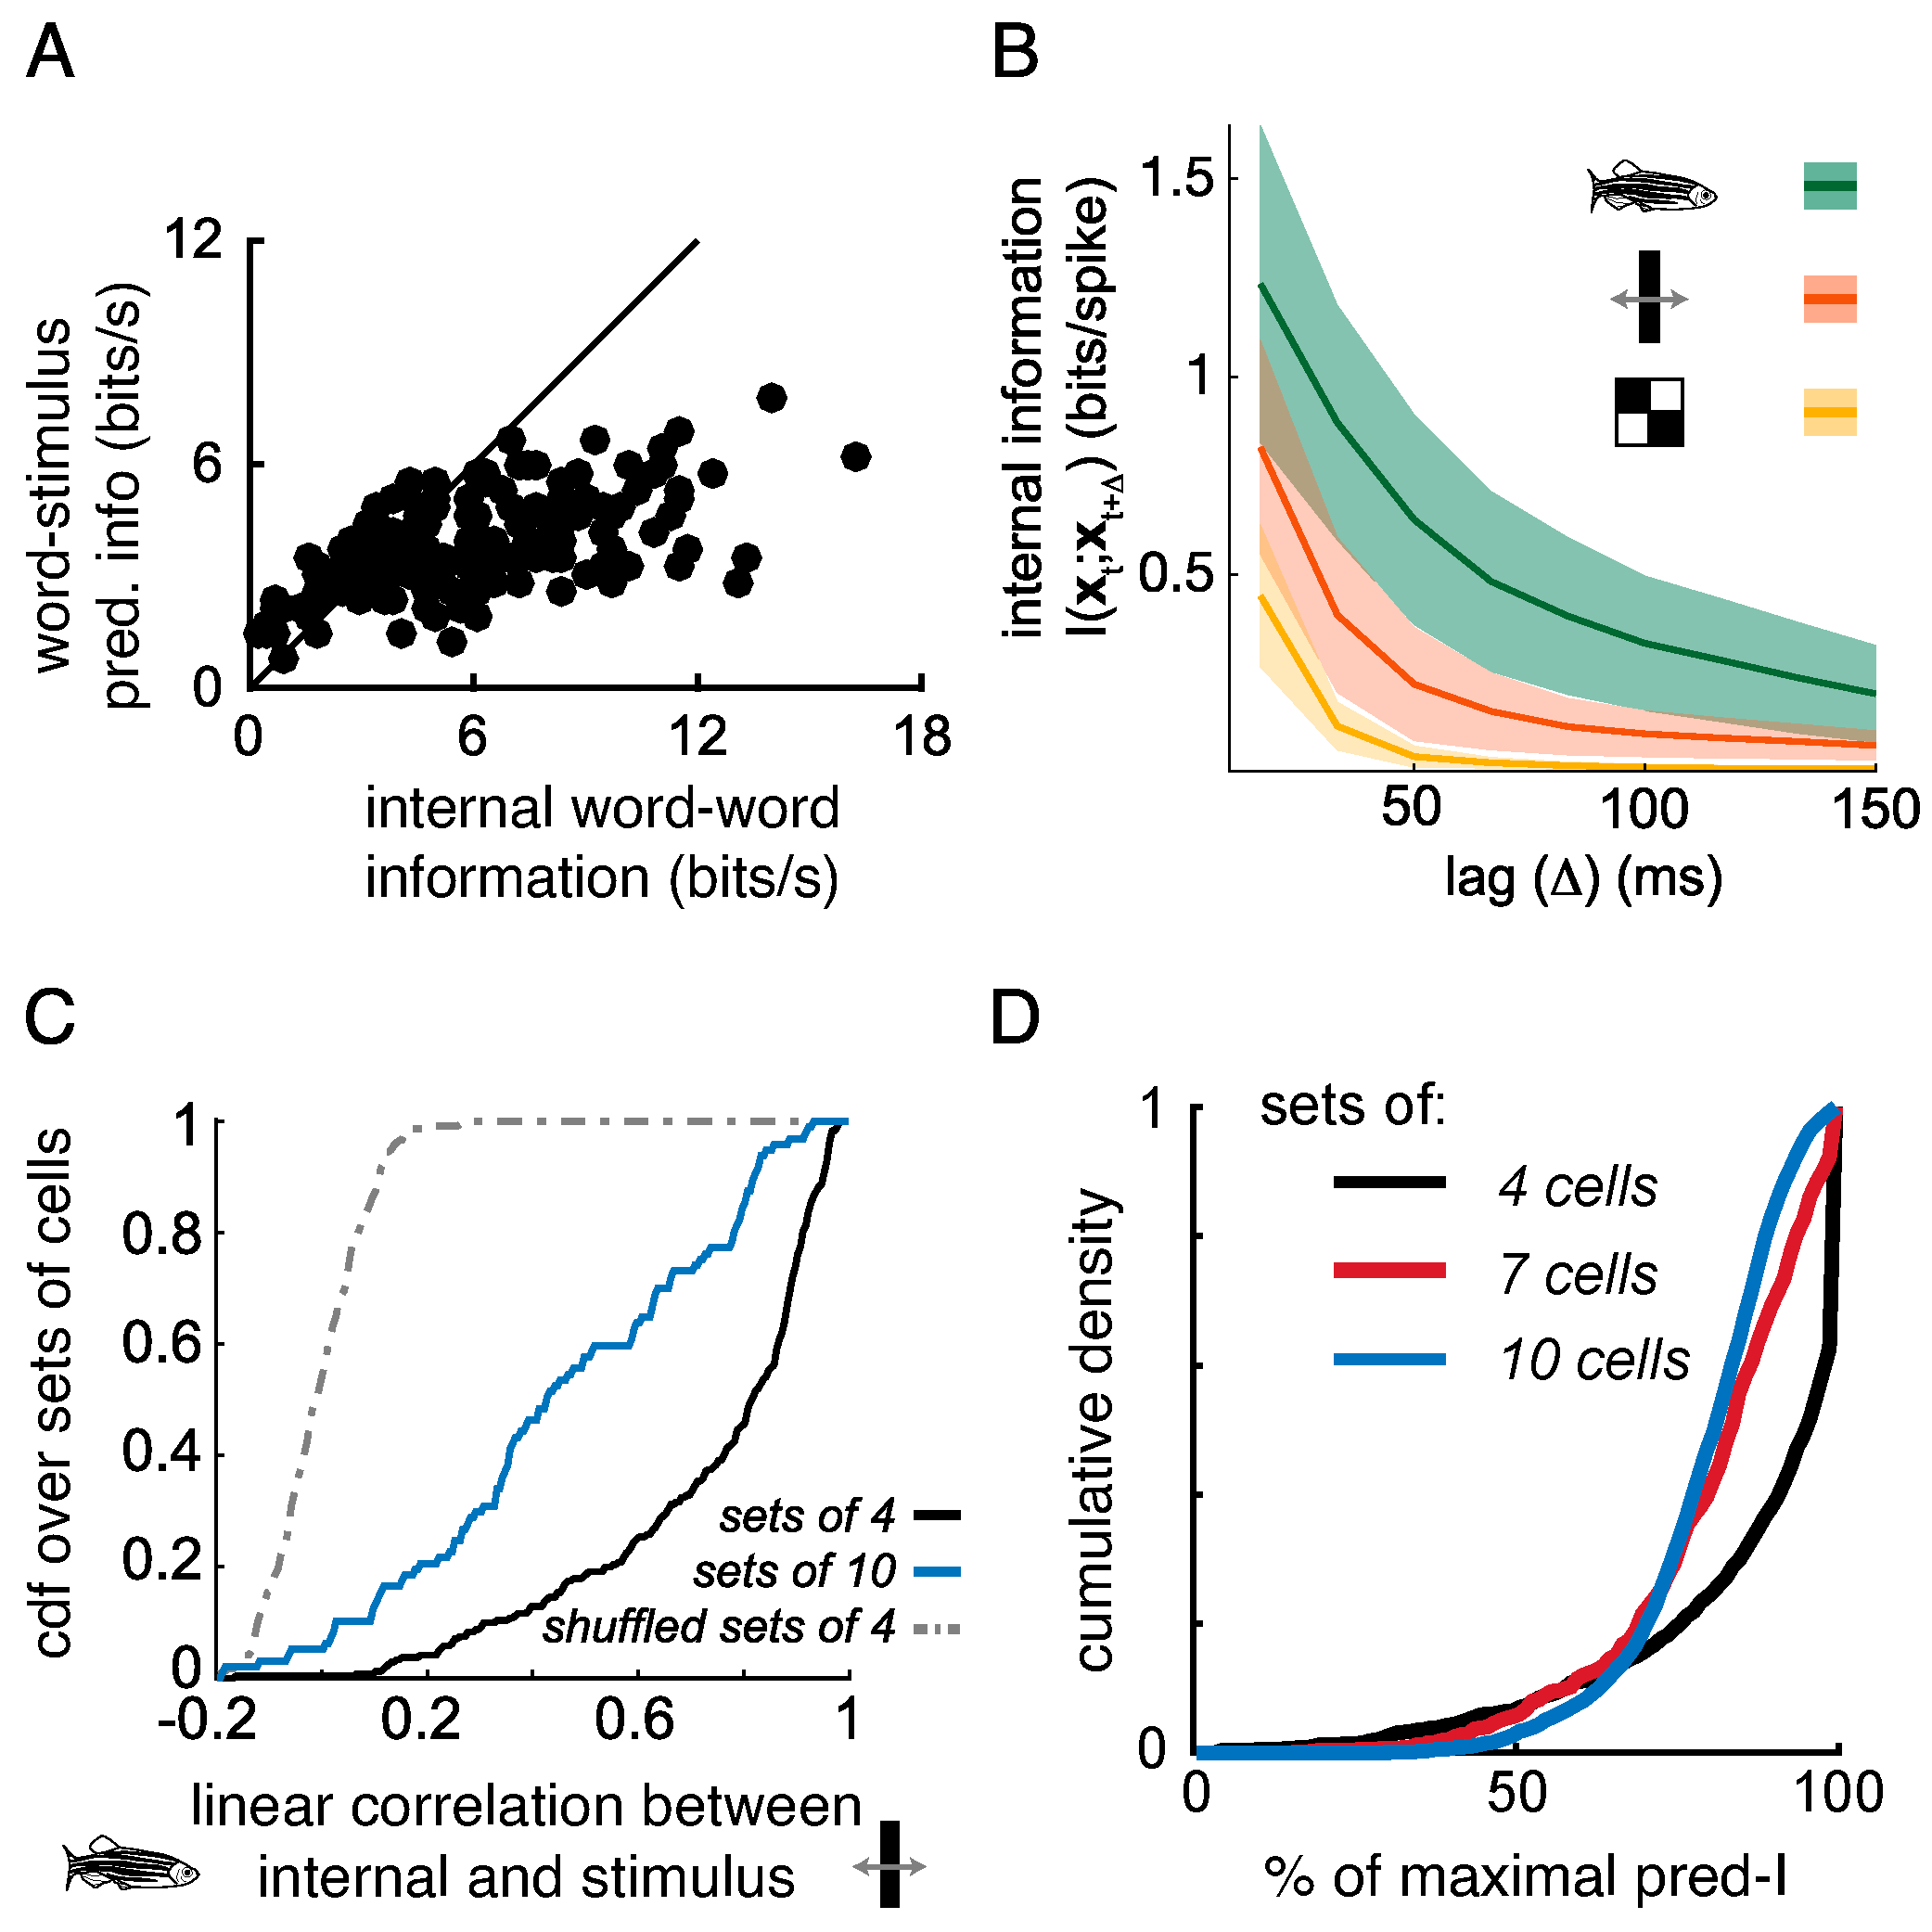
\includegraphics[width=\textwidth]{WritingMaterials/Fig_Sederberg/Fig_Sederberg.pdf}
            % 				\caption{Figure adapted from \cite{sederberg2018learning}}
            % 				\label{fig:sederberg2018learning}
            % 			\end{figure}


% ============================================================================ %
%                            Neural coarse-graining                            %
% ============================================================================ %
	\section{Coarse-graining in The Neural System} \label{sec:Neural coarse-graining}

		%% stochasticity at microscopic levels
		Despite the evolutionary advantage of having NTIC processes in a system, however, to create NTIC with a highly stochastic process is challenging. NTIC requires the predictability of the system state and is therefore impeded by noise in the system. Information processing at the microscopic levels (the cellular levels) in neural systems suffer from multiple environmental noise sources throughout, including sensory, cellular, electrical, and synaptic noises. For example, neurons have large trial-to-trial variability at the cellular level, and are subject to thermal fluctuations and other physical noises \citep{faisal2008noise}. 
		
        % 		Furthermore, environmental information is always only partially observable to individual sensors and neurons which only receive little amount of information from the environment. Therefore, information about the environment state at the cellular level is difficult to represent at the cellular level. It is implausible to construct NTIC processes at microscopic levels.

        %% Our argument
		However, we argue that, neural systems can form NTIC at certain macroscopic levels through coarse-graining microscopic neural states. Coarse-graining refers to many-to-one functions which aggregate microscopic states to a macroscopic state. In other words, a number of different micro-states realise the same value of the macro-variable \citep{price2007causation}. Neural systems, therefore, can form more stable and deterministic state transitions and be more capable of forming NTIC processes at certain coarse-grained macroscopic levels. 
		
		Indeed, empirical evidence has been showing that coarse-graining is a common coding strategy against ubiquitous stochasticity at microscopic levels of the the neural system. For instance, the inter-spike intervals of individual neurons are stochastic. This implies that states of individual neurons are incapable of encoding and representing stable information. However, the spiking rate, i.e. the average spike counts in a given time interval, shows astonishing stability and robustness against noise causing the variation of inter-spike intervals. Using this temporal coarse-graining strategy, known as rate coding \citep{adrian1926impulses, gerstner2002spiking, maass2001pulsed, panzeri2015neural, stein2005neuronal}, individual neurons can encode stimulus intensity by increasing or decreasing firing rate \citep{kandel2000principles}. \citep{stein2005neuronal}. The robustness of the rate coding is direct consequence of the many to one map used.
		
		% population code
		Population coding is another example of encoding information through coarse-graining in neural systems. In this coding scheme, information is encoded by activation patterns of a set of neurons (a neuron population). To reduce the influence noise on scholastic state transitions of individual neurons, many states for a neuron population map to the same information content. Therefore, stable representation can be formed through coarse-graining a high dimensional state space of a neuron population to a low dimensional state space of encoded contents \citep{kristan1997population, pouget2000information, binder2009encyclopedia, QuianQuiroga2009}. Therefore, individual neuron states (the microscopic level) are not informative about the encoded contents at the population level (the macroscopic level). Instead, coarse-grained variables are better entities to encode information and allow the neural system to ignore noisy causal interaction at the fine-grained level of description \citep{Woodward2007-WOOCWA}.
		
        The two examples show that coding schemes through coarse-graining could provides a stochastic system, e.g. the neural system, to form more stable and deterministic macroscopic processes to encode and process information reliably. We argue that through coarse-graining the neural systems is able to form NTIC processes at macroscopic levels. Based on this argument, we proposes our theory of consciousness in the next section. 


			
			
% 		% neural coarse-graining by Nic
% 		The practical implementation mentioned above suggests that  NTIC can be formed by coarse-graining sensory inputs in artificial neural networks. \citep{guttenberg2016neural} proposed a "neural coarse-graining (NCG)" architecture which aims to capture the emergent large-scale dynamics in the environment. The NCG network learns to coarse-grain input signals and extract latent variables which are both predictive and predictable in the input signal and therefore form NTIC.





% ============================================================================ %
% Boundary problem 1: Add another NTIC process
% 1. Ignore it / maybe next paper
% 2. Acknowledge the problem but we don't have solution now
% 3. Write down our comment 

% Micro/Macro and Environment point of views
%   Whether a process can be a part of the environment
% ============================================================================ %


% ============================================================================ %
%               A neural coarse graining theory of consciousness               %
% ============================================================================ %
	\section{A neural coarse graining theory of consciousness}\label{sec:OurTheory}
	

        In this section, we propose a new theoretical framework of consciousness: \acf{OurTheory}. We also discuss the implications of \ac{OurTheory} in Sec.~\ref{sec:cl}, \ref{sec:cc}, and \ref{sec:reconcile}.
        
        We argue that the existence of an NTIC process within a system is sufficient for information processing to be conscious.

        In what follows, we will first establish three assumptions on which this theory depends. Then, we will develop the propositions in detail. 
        
        The first assumption is that every human conscious precept is informative. Here, "informative" refers to the resolution of uncertainty. Being in a certain conscious state rules out a number of other possible conscious states. This is in line with the impression that our conscious experience consist of multi-dimensional information and usually involves information from multiple modalities. Therefore, every human conscious precept resolves some amount of uncertainty and provides information.  
        
        This assumption is also in agreement with one of the "axiom", \textit{information}, in Integrated Information Theory (IIT 3.0) which claims that \myQuote{...an experience of pure darkness is what it is by differing, in its particular way, from an immense number of other possible experiences...} \citep[p.2]{oizumi2014phenomenology}.
        
        Second, we further assume that all information requires physical substrates. 
        From these two assumptions, it follows that the amount of (self-)information possessed by a conscious percept must be equal to the (self-)information of a particular event or entity in the physical reality. 
        
        In this theory, we consider information is the common language between conscious experience and the physical reality. This means that consciousness is fundamentally associated with information \citep{chalmers1996conscious, tononi2004information, gamez2011information, Gamez2016}).
        
        The third assumption is that no consciousness can contain information of the entire universe. This means that there exists a informational boundary for every consciousness, i.e. informationally closed to the the universe. This is in line with our conscious experience that information provided by every conscious percept is limited.
    
        Together with the first three assumptions, this means that the physical representations of the contents of any consciousness must be a coarse-graining of the universe states and also informationally closed to the universe.
        
        Note that a coarse-grained process $Y$ can be a coarse-graining of another coarse-grained process $S$ of the universe $X$ (see Fig.~\ref{fig:fullgraph}). Here, we consider $S$ is a dynamic system and $Y$ is a coarse-grained process of the system $S$. Therefore, the environment $E$ of $S$ is also a coarse-graining of the universe. Importantly, in such case, if a macroscopic process $Y$ is informationally closed to the universe $X$, this implies $Y$ is also informationally closed to the microscopic level of the system $S$ and the environment $E$. 
    
		\begin{equation}
			\label{eq:ICchain}
			\begin{aligned}
		    & I(Y_{t+1};X_t|Y_{t})=0 & \implies & I(Y_{t+1};S_t|Y_{t})=0 \\
		    & {} & \implies & I(Y_{t+1};E_t|Y_{t})=0
			\end{aligned}
		\end{equation}
        
        This results in a crucial implication that informational closure can occur between levels in a system. The macroscopic level $Y$ can be informationally closed to the microscopic level $S$ within a system \citep{PFANTE.2014}.

		\begin{figure}[H]
		    \centering
			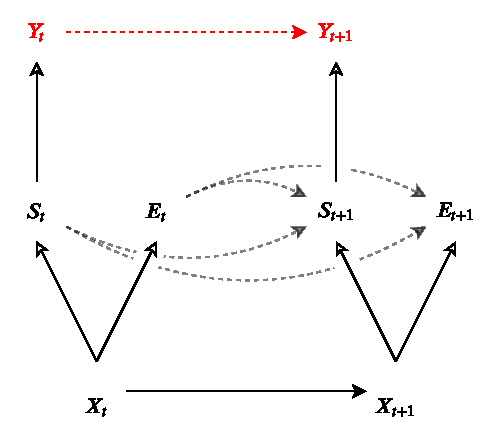
\includegraphics[width=\textwidth]{WritingMaterials/Fig_FullGraph/FullGraph.pdf}
			\caption{The information flow amounts the universe $X$, the system $S$, the environment of the system $E$, and the coarse-grained process of the system $S$. The solid line with a filled arrow from $X_t$ to $X_{t+1}$ represents the microscopic dynamic of the universe. The solid lines with a empty arrow represent directions of coarse-graining. The dashed lines represents virtual dependencies between  two macroscopic variables. The red $Y_t$, $Y_{t+1}$, and the red dashed line in between represents a macroscopic process which forms informational closure at a certain coarse-grained level.}
			\label{fig:fullgraph}
	   	\end{figure}
       
        A concrete example in the context of neuroscience is that $X$, $S$, $Y$, and $E$ represent the microscopic level of the universe, a cellular level process in the neural system, a macroscopic process of the neural system coarse-grained from the cellular level process $S$, and the environment which the cellular level process $S$ interacts with which may includes other processes in the neural system, the sensors for perception and interoception, and external physical worlds, respectively.	   	
        
        Our fourth assumption is that information provided by every conscious content is not trivial. More precisely, there exists a certain degree of mutual information between conscious processes and the environments which it interacts with. As mentioned in Sec.\ref{sec:Non-trivial informational closure} regardless one process is informationally closed to another one, to form mutual information between the two processes, i.e. NTIC, is still possible. Therefore, a macroscopic process $Y$ can be NTIC to the system's environment $E$ and concurrently be informationally closed to its microscopic process $S$. In other words, the macroscopic process can encode environmental information (by forming NTIC) and, however, be ignorant to its microscopic processes (IC). This is in line with our conscious experience that information that every conscious percept provides represent rich and structured environmental states without involving much information at microscopic activities.
        
        Finally, together with the four assumptions above, our main proposition is that the coarse-graining that physically represent consciousnesses are those that are informationally closed with respect to the universe states and concurrently be NTIC with respect to its environment. More formally this means that every NTIC process $Y_t$ at time $t$ corresponds to a conscious process $C_t=\{C_t^{Content},C_t^{Level}\}$ such that the content $C_{t}^{Content}$ of $C_t$ is just $Y_t$:
		\begin{equation}\label{eq:cContent}
			C_{t}^{Content} = Y_{t}.
		\end{equation}
		
		
		\noindent
        We further propose that the level of consciousness $C_{t}^{Level}$ can be measured by the degree of $NTIC_{t}$ of $Y_t$:
		\begin{equation}\label{eq:cLevel}
			C_{t}^{Level} = NTIC_{t}.
		\end{equation}
		We discuss the implications of these propositions in the following. 	
		
		
		% ---------------------------------------------------------------------------- %
        %        Level of Consciousness correlates degrees of NTIC of a process        %
        % ---------------------------------------------------------------------------- %
	    \subsection{Level of Consciousness is equal to the degree of NTIC of a process}\label{sec:cl}
            
            According to Eq.~\ref{eq:nticObjective}, \ac{OurTheory} implies that conscious levels are determined by two quantities. 
            
            First, to form high level of NTIC, one can increase the mutual information $I(Y_{t+1};Y_{t})$ between the current internal state $Y_t$ and the future internal state $Y_{t+1}$. In other words, conscious levels are associated with the degree of self-predictive information. This mutual information term can be further decomposed to two information entropy quantities: 
            
            \begin{equation}
            \label{eq:SelfEntropy}
            I(Y_{t+1};Y_{t}) = H(Y_{t+1}) - H(Y_{t+1}|Y_t)
            \end{equation}
            
            This implies that a high NTIC process should have a rich dynamic and concurrently maintain self-productiveness overtime. Another implication is that a complex systems can potentially reach higher levels of consciousness due to a larger information capacity to achieve higher mutual information. This outcome is consistent with a common intuition that conscious levels are associated with the degrees of complexity of systems.
    
    	    Second, one can minimise the conditional mutual information $I(Y_{t+1};Y_{t}|E_{t})$ to increase the level of NTIC. This quantity suggests that conscious level increases with the level of information about the environment state $E_t$ that the NTIC process encodes in its own state $Y_t$. An important implication is that a NTIC possessed by an agent which interacts with and adapts to a complex environment should have a higher level of NTIC than one possessed by another agent which lives and adapts to a simple environment. In other words, the environmental complexity is associated with conscious levels of NTIC processes.
    	   
    	    %% not monotonic
    		It is important to note that NTIC can be a non-monotonic function of the scale of coarse-graining. We saw above that not coarse-graining enough and therefore considering processes that are too microscopic leads to low values of NTIC. However, if the macroscopic variable is overly coarse-grained the system states can result in low degrees of NTIC. For example, in an extreme scenario, when all microscopic states map to a single macroscopic variable, the macroscopic level does not have any information capacity and thus looses the self and environmental predictive power. \ac{OurTheory}, therefore, argues that only processes at a certain level of coarse-graining in the neural system can reach high level of NTIC (Fig.~\ref{fig:LevelOfConsciousness}). As a result, there exists a certain level of coarse-graining which has a maximal conscious level within the neural system. 
    		
    		\begin{figure}[H]				
        		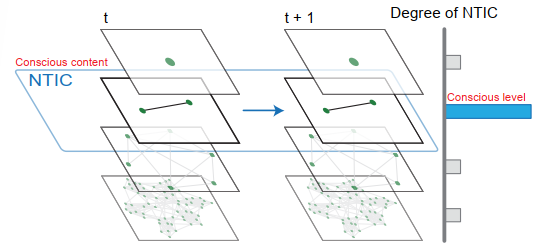
\includegraphics[width=\textwidth]{WritingMaterials/Fig_temp/FoxitReader_2019-01-31_19-03-59.png}
        		\caption{A n1on-monotonic relationship between Level of coarse-graining and level of consciousness.}
        		\label{fig:LevelOfConsciousness}
    		\end{figure}
            
            
            
            \ideaBox{About Human Scale}
            Finally, which coarse-grained level can form high NTIC? 
            agent-scale operation
            At the physical scale which human being interact with, the environmental dynamics is nearly deterministic following the laws of classical physics. It gives agents interact at this physical scale great advantages if the agents can build NTIC process internally. Therefore, to coarse-grain microscopic states is necessary
    	   
    
            %% Link to consciousness
            At the physical scale which human beings live in, the environmental dynamics is nearly deterministic following the laws of classical physics. This suggests that information in the environment is nearly closed at the right spatio-temporal scale. Therefore, this gives agents living at this physical scale great advantages if the agents form an NTIC process internally. Therefore, coarse-graining becomes necessary to map microscopic sensory and neuronal states into macroscopic NTIC process. 
            	   
    			
    
    
    
		\subsection{Conscious Contents Corresponding to States of a NTIC process}\label{sec:cc}
    	    % richness 
    		\ac{OurTheory} proposes that conscious contents correspond to states of NTIC processes (Eq.~\ref{eq:cContent}). This implies that the size of the state space of a NTIC process is associated with the richness of conscious contents that the process can potentially have. Therefore, a complex NTIC process with a high dimensional state space can have richer conscious experience than a simple NTIC process can have. This outcome is consistent with a the intuition that the richness of conscious contents is associated with the complexity of a system. 
    		
    		% CC doesn't include all microscopic states
    		As mentioned above, informational closure can happen between scales of coarse-graining within a single system. Thus, a macroscopic NTIC process can be ignorant to its microscopic states. \ac{OurTheory} argues that human conscious contents do not reflect cellular level activity because the conscious process which corresponds to a macroscopic NTIC process is informationally closed to the cellular level in the human neural system. Further more, since NTIC processes are informationally closed, each of them can be considered as a reality. In the extreme case, when the information flow from the its microscopic processes and environment is completely zero (Eq.~\ref{eq:informationflow2}), the future states of the process is only determined by its past states. 
    		
    		Importantly, NTIC processes encodes environmental information in its state. This suggests that a NTIC process can be considered as a process that simulates the environmental dynamics. This implication fit well with mental simulation theory of consciousness, predictive processing perspective of consciousness, and information generation theory of consciousness \needref{need three}. Note that \ac{OurTheory} doesn't assume that generative models are necessary. The implication a natural consequence based on our proposition. 
            
            Finally, due to a coarse-graining is a many to one map from microscopic to macroscopic scales, our theory implies multiple realisation thesis of consciousness\needref{multiple realisation} which suggests different physical implementation can map to the same conscious experience.
            
            
		% ---------------------------------------------------------------------------- %
        %             Reconciling the levels and contents of consciousness             %
        % ---------------------------------------------------------------------------- %
	    \subsection{Reconciling the levels and contents of consciousness}\label{sec:reconcile}
    	    Segregation of conscious levels and conscious contents raises a debate \citep{bayne2016there, Fazekas2016}. In \ac{OurTheory} conscious levels and conscious contents are just two different properties of NTIC processes, and, therefore, naturally reconciles the two aspects of consciousness. To form high NTIC, a NTIC process needs to have a large and potentially high state space which guarantees rich and high dimensional information in conscious contents. Therefore, this framework well integrates the two key but debated concepts in consciousness research
    	    
    	    
    	    According to Sec.~\ref{sec:cl} and Sec.~\ref{sec:cc}, an important implication from \ac{OurTheory} is that the the size of the state space and information entropy $H(Y)$ of a NTIC process are associated with both conscious levels and conscious contents. To reach high NTIC, a process needs to have a large state space and high information entropy which guarantee rich conscious contents and also the capacity of predictive information of the system (Eq.~\ref{eq:nticObjective}).
    	    \ac{OurTheory} therefore explains why in normal physiological states conscious levels and conscious contents are positively correlated \citep{laureys2005neural}. This implication is also in line with the intuition in which consciousness is often associated with complex systems.
    			
            % ---------------------------------------------------------------------------- %
            %                              Dynamical Boundary                              %
            % ---------------------------------------------------------------------------- %
            % \subsection{Dynamical Boundary}
            % Our theory predicts that the boundary of a conscious system is dynamical. The boundary is determined by the NTIC process. This implies that when the structure of interaction between variables changes the physical boundaries supporting consciousness should also change. If some coarse-grained variables encode environmental information, they may become necessary components to form high NTIC. In such case, these coarse-grained variables are "recruited" inside the boundary of conscious processes. Note that, due to synergistic information, even recruiting some new variables may largely increase the level of NTIC. 
            % This may explain why consciousness is tightly associated with binding and integration of information in human perception and cognition. Another crucial implication is that the same neural substrates may not be always involved in conscious processing rather it depends on whether it creates high NTIC with other members in the neural system. \needfig{Maybe I need a figure here as well}
    
    
% ============================================================================ %
%                    Conscious versus Unconscious Processing                   %
% ============================================================================ %
	\section{Conscious versus Unconscious Processing}\label{sec:Conscious versus Unconscious Processing}
	    In this section, we show how our theory can make predictions about what processes are conscious and what are unconscious. 
	    
        % While our theory is built upon a minimal set of assumptions, it possesses predictive power about the relationship between information processing in the neural system and conscious experience.
	    
        % 		Our theory argues that, to make information conscious, the following necessary and sufficient conditions need to be satisfied.
        
        %         We especially highlight the second condition because it is critically related to many empirical research results even though it is only a necessary condition. As we will describe below, this theory can well explain a variety of previous empirical findings in consciousness science and further make predictions for future research. In this section, we discuss how the two informational-based conditions link to conscious experience. 
		
		
		
        % ---------------------------------------------------------------------------- %
        %                            Unconscious Processing                            %
        % ---------------------------------------------------------------------------- %
        \subsection{Unconscious Processing}
            \ac{OurTheory} proposes that NTIC is sufficient for a process to be conscious. Based on the definition of NTIC, we highlights two scenarios which lead low NTIC so that a process is unconscious. We additionally highlight the level of coarse-graining.
            \ideaCallout{Need rewording}
        
        
            % ============================================================================ %
            %                                 Fail to be IC                                %
            % ============================================================================ %
            \subsubsection*{Fail to Form Informational Closure}
                A process is not informationally closed leads to low levels of NTIC (Eq.~\ref{eq:nticObjective2}) and results in low or no consciousness. In this case, the current states of a process are largely depends on its environment states (see Fig.~\ref{fig:reflexive}) but little influenced by its past states. Reflexive behaviours \citep{casali2013theoretically} can be considered a classical example in this scenario. \ac{OurTheory} naturally explains why reflexive behaviours always do not involve voluntary conscious controls and operate unconsciously. 
         
             	% reflexive behaviour
        		\begin{figure}[H]
        			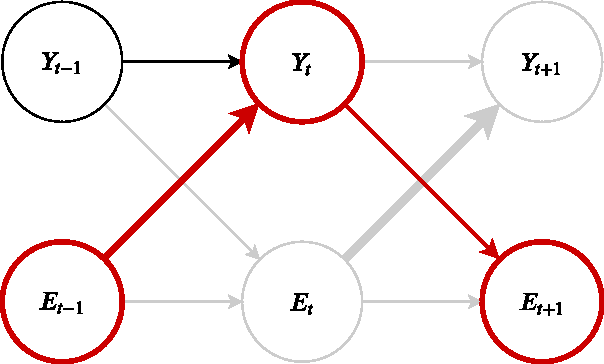
\includegraphics[width=0.8\textwidth]{WritingMaterials/Fig_Reflexive/Reflexive.pdf}
        			\caption{
        			    Reflexive behaviours happen between a process $Y$ and its environment $E$ which $Y$ interact with. The red nodes and arrows represent the major information flow in reflexive reactions. The internal state of the process $Y_t$ is largely dependent on the environment state $E_{t-1}$ but less on its past state $Y_{t-1}$. Therefore, the process $Y$ is not informational closed. In consequence, $Y$ is unable to form high NTIC and, therefore, to have high conscious levels.
        			    }
        			\label{fig:reflexive}
        		\end{figure}  
        		
        		The same principle can be applied to blindsight \citep{humphrey1999history, humphrey1974vision, Humphrey1970} and procedure memory \citep{doyon2009contributions, ashby2010cortical} which are often considered as unconscious processes. Blindsight patients are able to track objects, avoid obstacles, and make above chance-level visual judgements without having any conscious perception about visual stimuli. We argue that action outputs of blindsight can be directly guided by sensory inputs through stimulus-response maps. The neural circuits are not informationally closed and, therefore, unconscious. Similarly, for procedure memory, the state transitions of action controls largely depends on the concurrent environmental states. This prevents the internal processes of procedure memory from informational closure and being conscious. 
         
                % In the neural system, this type of processes, for perception, shows the property that the perceptual processing mainly passively responds to the sensory inputs. For actions, this type of processes only produces "reflective-like" behaviours. Reflexive behaviours are commonly considered as automatic and non-conscious behavioural controls \citep{casali2013theoretically}\needref{More referene}. We argue that information carried by this type of processes is unconscious due to its failure of achieving high NTIC, i.e., the first condition. 
                
                % The same principle can be applied to blindsight and procedure memory \needref{blindsight} which are often considered as unconscious processing. Blindsight patients are able to track objects, avoid obstacles, and make above chance-level judgements without having any conscious perception about visual stimuli. We believe that these behaviours can be guided by direct stimulus-response mappings ($S\rightarrow{}R$). However, the direct $S\rightarrow{}R$ mappings also lead to non-NTIC neural processes  and, therefore, are unconscious. Similarly, in the case of procedure memory, processes always rely on both the current environmental and system states to determine the next state of the processes\needref{Do I need ref??}. The information flow from the environment to the system is crucial to guide the state transition of procedural memory. Therefore, information processing of procedural memory also fails to form high NTIC and remain unconscious. 
                
        %          This type of processing is similar to the model-free policy-based agents in the reinforcement learning framework. The agent learns a policy $\pi$ which directly maps sensor values $S$ to output action $A$.
        % 		\begin{equation}
        % 			\label{eq:PolicyBasedAgent}
        % 			\begin{aligned}
        % 			    \pi(A | S)=\operatorname{Pr}\left(A_{t}=a | S_{t}=s\right)
        % 			\end{aligned}
        % 		\end{equation}
        		
                \ac{OurTheory} explains why the patients with visual apperceptive agnosia \citep{james2003ventral} can perform online motor controls without visual awareness of action targets \citep{10.3389/fneur.2014.00255}. The online information from the visual inputs can be used to perform  functional actions without complete conscious perception of the visual targets. 
                
                
                % Our theory also explains why unconscious processes in this category often fail when a long delay periods is introduced in the tasks. Without self-predictive information in NTIC, the policies of motor outputs largely depends on the present environmental and sensory states implying that this type of processes often can only work online. With a long, sensory information is unable to guide the delayed motor outputs and leads to failure consequences. 
        		
        		\ideaCallout{Mayeb can put in theory part}
        		An implication from \ac{OurTheory} is that a pure feedforward network is incapable to be conscious due to a lack of any form of memory. Without memory, the network current states are entirely driven by network current inputs without any influence from its past states and, therefore, is incapable to be informationally closed. In contrast, a network with recurrent loops could keep information about its states. This forms an information channel between the past and the future states of the network and, thus, makes the network becomes capable of being informationally closed. This result coincides with theories of consciousness emphasising the importance of recurrent circuits to consciousness \citep{lamme2006towards, edelman1992bright, tononi2008neural}.
        		
        % 		However, we derive this conclusion from a more fundamental informational-related hypothesis indicating the more generalised principle behind it. 


            \subsubsection*{Encoded Information is Trivial}
                Encoded information in a process is trivial, i.e. no mutual information between the system states and its environment states $I(Y_{t+1};E_{t})$ (Eq.~\ref{eq:nticObjective2}), could also lead low NTIC. This process is considered to be unconscious due to the low level of NTIC. This implies an isolated process which is simply informationally closed to its environment is not enough to be conscious. 
                
                This implies that \ac{OurTheory} provides a natural solution to the boundary problem of consciousness \citep{Raymont2006-RAYUOC}. Consider a NTIC process $Y$ and an isolated informationally closed process $\hat{Y}$ with trivial information. Adding $\hat{Y}$ to $Y$ can still keep informational closure, but, however, does not increase non-trivial information. 
                
    			\begin{equation}
    			    \begin{aligned}
                        I(Y,\hat{Y};E) & = H(Y,\hat{Y}) - H(Y,\hat{Y}|E) \\
                                       & = H(Y) + H(\hat{Y}|Y) - (H(Y|E)+H(\hat{Y}|Y,E)) \\
                                       & = H(Y) + H(\hat{Y}) - (H(Y|E)+H(\hat{Y})) \\
                                       & = H(Y) - H(Y|E)\\
                                       & = I(Y;E)				
    				\end{aligned}
    			\end{equation}
                
                This indicates that isolated processes with trivial information do not contribute consciousness and should be outside the information boundary of the conscious processing. This result also implies that consciousness does not emerge from aggregating informationally closed processes with trivial information. 
            
            % \ideaCallout{Should I say this?}
%             This implies that \ac{OurTheory} provides a natural solution to the boundary problem of consciousness \citep{Raymont2006-RAYUOC}. Consider a set of independent processes $Y=\{Y^1,...,Y^n\}$ with deterministic state transitions in a small universe. Each variable not only is informationally closed to other variables, they also share no mutual information.
            
% 			\begin{equation}
% 				\thickspace Y^i \bot Y^j, \quad \forall {i\neq j}
% 			\end{equation}
            
%             Now we randomly pick two variables and make group two variables s
            
%             , therefore, unconscious. Next, we can select a two of the variables and compute NTIC between this subset and other variables. 
        
        
            \subsubsection*{Unsuitable Measurement scales }
                \ac{OurTheory} proposes that human conscious process rests on a certain scale which forms NTIC. This implies the spatial and temporal scales of the physiological measurements are critical in the experiments aiming to finding neural correlates of consciousness (NCC).
            
            
                % \subsubsection*{Fail t  o meet the 2\lowercase{ed} condition}
                As mention above, information is level-dependent and can be virtually independent (closed) across different coarse-graining scales. If processes at some levels of a system are able to form high NTIC and become conscious, information at other levels still remains unconscious. The first implication of this argument is that processes at levels with high stochasticity are unable to form high NTIC and, therefore, unconscious. High stochasticity corrupts informational channel capacity and leads to low mutual information between past and future states of a process. In the neural system, the cellular level activities are highly noisy and are unable to reach high NTIC. Therefore, the information processed by the microscopic levels in the neural system are not conscious and we never can experience detail activities in the microscopic levels. 
                
                
                We argue that many mysterious results in previous research of consciousness are originated from inappropriate biological and behavioural measurement scale. In the following, we list some examples. 
                
                
                Unconscious processing in this category of 
                
                @ Evidence suggests that the neural system is able to encode probability distribution and perform probabilistic inference in a near optimal way\needref{bayesian brain}. However, an intriguing fact is that we are nearly ignorant of all the probabilistic computation of the inference processes but are only aware of "a sample" of the posterior distributions of the inferences \citep{dehaene2017consciousness, vul2009attention, asplund2014attentional, vul2008temporal, moreno2011bayesian}. The information of all alternative possible states is unable to enter conscious contents. In short, one needs to explain why the neural system can hold the joint probability distributions of inferred variables but, however, only a realisation of the inference outcome becomes conscious. Based on our theory, we argue that the computation of statistical inference is carried out at microscopic levels of the neural system and the NTIC process correlated with conscious contents only possesses the coarse-grained information of the computation. The mapping from the microscopic to macroscopic states naturally leads to a single and stable state at the macroscopic levels.
                
                For example, Fig.~ \ref{fig:TemperatureExample} illustrates the relationship 
                At the left panel, two cups contain water with different volumes $V_t$ and temperatures $T_t$. Even though we know volumes and temperatures are coarse-grained macroscopic variables, the states of mixed water ($V_{t+1}$, $T_{t+1}$) can still be predicted without knowing any information from the microscopic levels (the molecular level),i.e., the information closure at the macroscopic level. Similarly, taking Bayesian inference as an example, the microscopic neuron populations are able to represent probabilistic distributions about inferred target variables and the neural networks perform the statistical inference to obtain the posterior distributions. However, enormous microscopic neural states can be coarse-grained into the same state of summary statistics (e.g., the mean $\mu_{t}$  and standard deviation $\sigma_{t}$) at a macroscopic level. The state transition ($\mu_{t+1}$ and $\sigma_{t}$) is also predictable without any additional information from microscopic levels. Therefore, consciousness can only "observe" the coarse-grained states without the knowledge of how the statistical inference is implemented and performed at the microscopic levels. 
        
        
        		\begin{figure}[H]
        			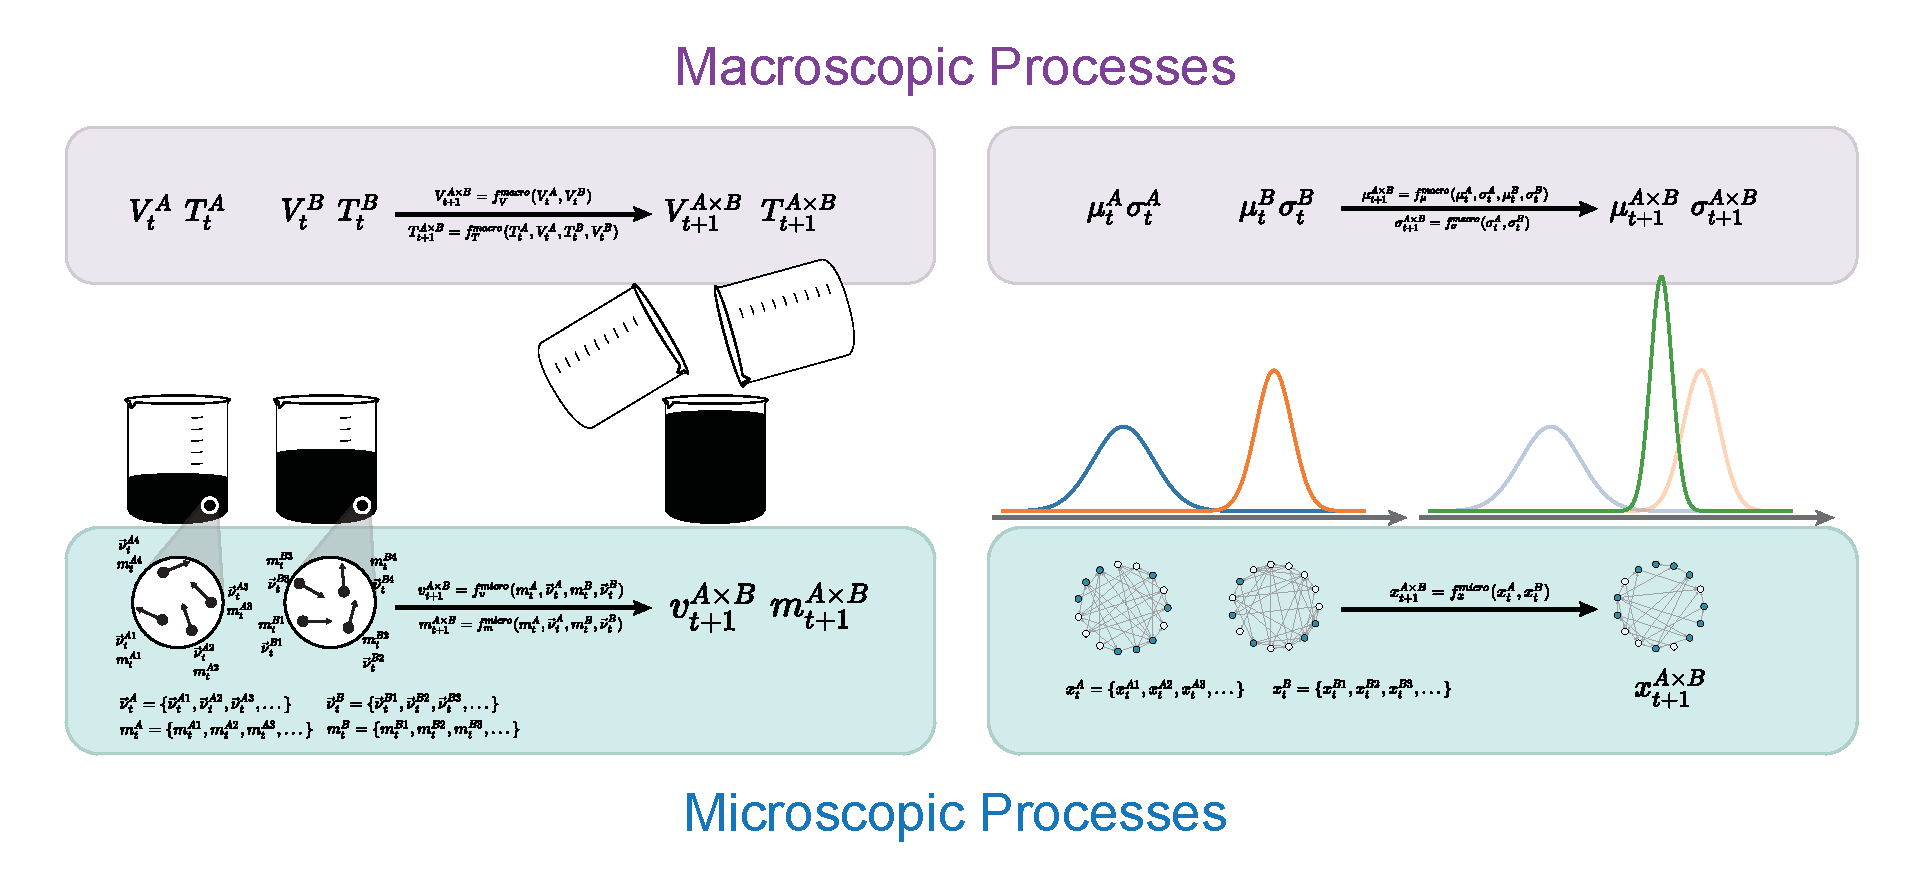
\includegraphics[width=1.3\textwidth]{WritingMaterials/Fig_Temperature_Example/ExampleOfCG.pdf}
        			\centering
        			\caption{An Example of ...}
        			\label{fig:TemperatureExample}
        		\end{figure}         
                
                
                The same scenario can be applied to the results from Libet's volition experimental paradigm \citep{Libet1983TimeOC, Libet1985Dec}. Experiments using similar procedures usually show that the recorded neural activities start earlier than subjects' feeling of their own intention to act in the self-determined experimental settings. We argue that free actions are initiated at the microscopic levels, for example, the random fluctuation in the neural system \citep{schurger_accumulator_2012}. However, the conscious experience of volition is information at the macroscopic level with NTIC. Due to the information closure, there is no way for the NTIC process to observe the information of the microscopic states, i.e. the initiation of actions. 
                
            
                \idea{Not sure if I want to address this point}  Note that, some evidence suggests single-cell-level correlation of conscious experience, the Jennifer Aniston cell for example \citep{Quiroga2005Jun, Quiroga2012Jul}. This may seem to counter our argument that single-cell level information is incapable to be conscious. However, first, the correlations are always not the direct microscopic state changes of the cells, e.g. the action potentials. Instead, the correlated variables are always coarse-grained. The neuronal firing rate, for example, is a temporal coarse-grained variable. Second, it has been well established that heterogeneous nonlinearity is critical for neural populations to encode rich and high dimensional information. \citep{Chelaru2008, Rigotti2010Oct, Shamir2004Jun}. It is common to detecting a single neuron whose activity profile well align with a subspace which represents a single object within the state space of a population code.\needhelp{Maybe need to rewording here} We believe that multi-scale data and analyses are needed to elucidate whether single neuron behaviours are sufficiently representative for any type of conscious experience. 
    

        

        % ---------------------------------------------------------------------------- %
        %                             Conscious Processing                             %
        % ---------------------------------------------------------------------------- %
		\subsection{Conscious Processing}
		When the both conditions are fulfilled, our theory suggests that the states of an NTIC process correspond to particular conscious contents and the information incorporated in the NTIC process is conscious. Due to the predictive nature about the environment dynamics of NTIC processes, to form high NTIC and to construct functions within the process have a huge evolutionary advantage. It is important to emphasise that our theory does not suggest any functionalism of consciousness. Rather, we argue that information fundamentally associates with consciousness. Nevertheless, consciousness research still suggests a strong functional relation between consciousness and some specific types of cognition and behaviours \citep{Seth2009Encyclopediaofconsciousness}. We believe that this relation comes from several special properties of NTIC and these properties support the foundations of many cognitive functions in the neural system.
		
		First, an NTIC process encodes predictive information about environmental dynamics. This is crucial for constructing forward models for predicting future states of the environment. Therefore, cognitive functions which require agent-scale prediction are likely to be accompanied by conscious experience. This properties is required by planning and also achieving long term goals.\needref{}
		
		Second, an NTIC process can be considered as a close form simulation machine. With a given initial state, the process can self-evolve and follow a certain trajectory in the state space. This trajectory can be seem as a simulation about the environmental transition. Therefore, an NTIC process can serve cognitive functions as a perfect simulation engine \citep{BERTSCHINGER.2006}. Accordingly, mental simulation, imagination, computing alternative realities, and generating counterfactual outcomes can be implemented with an NTIC process. \needref{}
		
	    Third, an important properties of NTIC processes is its high stability. The state transitions and trajectory are highly predictable. In such case, NTIC processes are more suitable for integrating information across larger time scales (above millisecond). Therefore, tasks which require to integrate information across time above the millisecond scale are often associated with conscious experience. 
	    
	    Fourth, an NTIC process as a closed system can still provide predictive information without new information flowing into the process. This is crucial for many types of off-line processing. 
	    
	    Fifth, any state of an NTIC process can be seem as a integration of multiple sources of information. For the human scale activities, to know certain transition about the environment, the NTIC process must include a high dimensional information from multiple modalities and have the knowledge about how the high dimensional data interact to each other. Without the knowledge and information, a process may not be capable of produce a stable state transitions which mimic the environmental dynamics. Thus, cognitive functions requiring this large scale integration are likely to be conscious. Furthermore, the high dimensional integrated information is also critical for an agent to learn new behaviours to achieve flexibility and the strategic behavioural controls and decision-making. 
	    
	    In sum, we argue that having an NTIC process is critical for survival in the evolution. It is likely that biological creatures acquired NTIC process at some stages in the evolution. And due to the fundamental relationship between information and consciousness, these biological agents also acquired different degrees of consciousness depending on the physical scales and the complexity of the environments they live in. Our theory well explains why some processes and functions in the neural system are conscious and some are not with only two parsimonious conditions. 
	    


% ============================================================================ %
%                        Comparison with other theories                        %
% ============================================================================ %
	\section{Comparison with other Relevant Theories of Consciousness}\label{sec:Comparison with other theories}
	In this section, we \ac{OurTheory} with other relevant modern theories of consciousness.
	
	
        % ---------------------------------------------------------------------------- %
        %        Theories about multilevel views on consciousness and cognition        %
        % ---------------------------------------------------------------------------- %
        \subsection{Multilevel views on consciousness and cognition}
    		\ac{OurTheory} proposes that a conscious (NTIC) process only rest at a certain coarse-grained scale in the neural system. This suggests that the scales of coarse-graining is critical for searching for conscious processes. In previous research, a few multilevel views on consciousness have been (explicitly or implicitly) proposed. So far, to our knowledge, Pennartz's neurorepresentational theory (Neurorepresentationalism, \cite{pennartz2018consciousness,pennartz2015brain}) is the closest proposal in line with our multilevel view on consciousness. Similar to Neurorepresentationalism, the concept of levels \ac{OurTheory} is also relevant to Marr's level of analysis \citep{marr1982vision, pennartz2015brain, pennartz2018consciousness}. 
    		However, \ac{OurTheory} suggests that coarse-graining is necessary only when the microscopic processes are stochastic (e.g. the neural system). An NTIC process can be formed in a noise-free deterministic system without coarse-graining. According to \ac{OurTheory}, this NTIC process is sufficient to be conscious. 
    		Another fundamental difference between \ac{OurTheory} and Neurorepresentationalism is that Neurorepresentationalism takes functionalist perspective and suggests consciousness should serve high-level world-modelling and makes a best guess about the interaction between the body and the environment. 
    		%Neurorepresentationalism also suggests conscious experience is associated with integrated representation for multimodal and situational information.
    		However, \ac{OurTheory} is grounded by non-functional informational assumptions. Therefore, \ac{OurTheory} provides a more fundamental explanation for the scale problem of consciousness. 
    		
    		Another proposal based on multilevel views is the Intermediate Level Theory of Consciousness \citep[ILT]{prinz2007intermediate, jackendoff1987consciousness}. ILT proposes that conscious experience is only associated with representations at intermediate levels of the sensory processing hierarchy (e.g., the 2.5D representation in terms of visual processing) rather than lower (e.g. pixel) or higher (e.g. abstract ) levels of the hierarchy. 
    		Here, we want to make a clear clarification that the "level" in \ac{OurTheory} refers to the levels of coarse-graining instead of the "level" for anatomy or information processing. It is important to note that the coarse-graining direction is not necessary aligned with the levels of anatomy or the information processing hierarchy in the neural system . Our theory is different from consciousness theories which focus on the anatomical hierarchy, for example 
    		
    		
    		
    		specific levels of representations in the hierarchy of sensory processing. ILT claims that consciousness only associates with the representation at intermediate levels (e.g., the 2.5D representation in terms of visual processing) rather than the ones at lower-level or higher-level. 
    		
    		
    		One fundamental difference between ILT and our theory is the definitions of the level. In our theory, level is within the context of coarse-graining. However, ILT focuses more on the levels in terms of anatomical direction (see fig \ref{fig:hierarchy}). As mentioned previously, we emphasise that we doesn't assume the direction of coarse-graining should align with the direction of anatomical processing levels along cortical hierarchies. This leads to an important difference that the level of coarse-graining exists virtually. However, the level of cortical representation should be referred to neural substrates. Finally, different from ILT which suggests that some neural substrates responsible for the 2.5D computation are conscious, we predict that once information carried by coarse-grained variables is involved in the NTIC process, brain areas, not exclusively within 2.5D representation, should  co-vary with conscious contents. 
    		
    		
            
    			
        % ---------------------------------------------------------------------------- %
        %                 sensory hierarchy and neural coarse-graining                 %
        % ---------------------------------------------------------------------------- %
		\subsection{sensory hierarchy and neural coarse-graining}\label{sec:SensoryHierarchy}

        It is important to note that the coarse-graining direction is not necessary aligned with \critical{Just saying anatomical is not enough. Need better expression} anatomical sensory hierarchy in the neural system. Our theory is different from consciousness theories which focus on the anatomical hierarchy, for example 
        
        the intermediate Level Theory \citep[see also \ref{IntermediateLevelTheory}]{prinz2007intermediate, jackendoff1987consciousness}. Due to the pervasive noise in the microscopic levels in the neural system reliable information processes need to be built upon the coarse-grained levels. In figure \ref{fig:hierarchy}, the blue arrows indicate the readout mechanisms implemented in the neural system. We argue that previous data suggesting the neural correlates of consciousness between microscopic neural activities and conscious contents may be misled. 

        
		\begin{figure}[H]
		
			\includegraphicsTodo[width=\textwidth]{WritingMaterials/Fig_SeperationOfCGandCortHierachy/SeperationOfCGandCortHierachy.pdf}
			\label{fig:hierarchy}
		\end{figure}
    


                \subsubsection*{Level of Organisation \cite{wimsatt1994ontology}}
                    As mentioned previously, the level of coarse-graining is different from the anatomical level.
                    Pennartz focuses more on multimodal representation as the most important factor (See the discussion in \cite{pennartz2015brain}). Our proposal is inline with Pennartz's Neurorepresentational  theory (Neurorepresentationalism) \cite{pennartz2018consciousness,pennartz2015brain}. However, it’s crucial to note that our theory claims only the level of coarse-graining achieving NTIC matters to consciousness rather than the anatomical level of sensory hierarchy. 
    
    			\subsubsection*{Intermediate Level Theory} \label{IntermediateLevelTheory}
                    One important theory tries to connect consciousness to multilevel views is the Intermediate Level Theory (ILT, \cite{jackendoff1987consciousness, prinz2007intermediate}). ILT proposes that conscious experience only correlates specific levels of representations in the hierarchy of sensory processing. ILT claims that consciousness only associates with the representation at intermediate levels (e.g., the 2.5D representation in terms of visual processing) rather than the ones at lower-level or higher-level. 
                    One fundamental difference between ILT and our theory is the definitions of the level. In our theory, level is within the context of coarse-graining. However, ILT focuses more on the levels in terms of anatomical direction (see fig \ref{fig:hierarchy}). As mentioned previously, we emphasise that we doesn't assume the direction of coarse-graining should align with the direction of anatomical processing levels along cortical hierarchies. This leads to an important difference that the level of coarse-graining exists virtually. However, the level of cortical representation should be referred to neural substrates. Finally, different from ILT which suggests that some neural substrates responsible for the 2.5D computation are conscious, we predict that once information carried by coarse-grained variables is involved in the NTIC process, brain areas, not exclusively within 2.5D representation, should  co-vary with conscious contents. 
    				
	
        
        % ---------------------------------------------------------------------------- %
        %                                      IIT                                     %
        % ---------------------------------------------------------------------------- %
		\subsection{Integrated information theory}
    		Integrated information theory (IIT) states that system's consciousness is determined by its causal properties. Consciousness is integrated information. As a computational theory of consciousness, the degree of discrimination and integration can be expressed in mathematical terms $\Phi$. Different from most of other scientific theory of consciousness, IIT asserts that the fundamental physical property associated with consciousness is causality.
    		
    		% -------------------------------- Similarity -------------------------------- %
    		IIT and our theory shares common principles in many aspects. First common principle between our theory and IIT is that instead of NCC, both theories suggest information is the fundamental entity which correlates consciousness \needref{cite David Chalmers}. Therefore, both theories are capable of extrapolation and infer the states of consciousness in other systems beyond the human neural system.
    		
    		Second, both theories consider informational structure as the fundamental entities associated with the quality of conscious contents. IIT proposes that a "complex" which is defined as elements that generates a local maximum of integrated information as the core entity which determines the state space of subjective feeling (qualia space). In the current stage of our theory development, we have not proposed such sophisticated description of the mappting between informational structure and the qualia space. However, in line with this notion, we argue that the state space of an NTIC process determines the subjective experience possessed by the process. 
    		
    		
    		
    		\ideaBox{Maybe synergy is the common part of the two theories }
    
    		Even though both theories are based on informational properties of a process, predictions of the two theories can be very different. Taking the split brain cases as the example, when splitting a system into two parts, IIT suggests that each part can form a new complex. Therefore, splitting creates two new conscious entities. However, according to our theory, splitting a system may totally destroy the informational structure that created NTIC. This may lead to very small degree of NTIC in both hemispheres, thereby entirely destroying consciousness of this system. Notwithstanding, more simulation work is needed to thoroughly clarify how the two theories make same and different predictions in different contexts. Fortunately, due to the computational nature of the two theories, precise differences of predictions can be made from relatively simple toy model in the future work. 
    		
    		% Hoel's theory\cite{hoel2016can}}
    		Alongside with the main theoretical development of IIT, \cite{hoel2016can,hoel2013quantifying} discussed the scale-dependent causal structures using IIT as a measure of causal power at different scales. The result shows a qualitative similarity to our theory. The causal power can emerge at macroscopic levels of a system. This claim is consistent with our prediction in which processes at macroscopic levels can form more deterministic and predictive state transitions. We expect further mathematical and empirical analysis can reveal the relationship between \ac{OurTheory} and Hoel's analyses about the causal power at different scales in a system.  
    		
            % =============== Internal simulation and self-modelling theory ============== %
    		\subsection{Internal simulation and self-modelling theory}
    		\idea{I will skip this section unless you think this is necessary.}



        % ---------------------------------------------------------------------------- %
        %                            Predictive Processing                             %
        % ---------------------------------------------------------------------------- %
		\subsection{Predictive Processing}
    		Predictive processing is a powerful framework (PP) which integrates several influential ideas in the history of neuroscience including "perception as unconscious inference" from Helmholtz \citet{helmholtz1866concerning}, "analysis by synthesis", “predictive coding”, and "Bayesian brain hypothesis". This emerging theoretical framework of perception and brain function suggests that the neural system constantly generates predictions about incoming sensory signals and updates predictions based on prediction error between predictions and real sensory signals. According to PP, the neural system constantly performs unconscious statistical inference about hidden causes in the external environment. The perceptual contents are the "best guess" about the environment states including these hidden causes \citep{clark_2013, Hohwy2013}. Because it is well integrated with Bayesian brain hypothesis, the PP has been used to interpret conscious perception in many perceptual domain. \cite{Hohwy2013} \cite{SethPP2014}.
    		
    		
    		%% The gaps between pp and consciousness
    		PP is a powerful explanatory framework for diverse brain functions. However, to serve as a theory of consciousness, PP is still incomplete due to two theoretical gaps. First, there are enormous predictive mechanisms in the neural systems. It is  obvious that that not all the predictive information from these mechanisms is able to be part of conscious contents. Therefore, PP needs to explain the difference between conscious and unconscious predictive mechanisms. Second, if we closely look at a conscious predictive system, the only part can be consciously aware of is the result. Other details of the computation remain unconscious. PP also needs to explain how unconscious inferences is able to give rise to conscious results. In short, the two explanatory gaps prevent PP from been a complete theory of consciousness. 
    		
    		Here, from more fundamental principles, we  argue that our theory is able to well fill the two gaps simply by considering the two conditions mentioned in section \ref{sec:Conscious versus Unconscious Processing}.
    		
    		First, predictive processes do not necessitate NTIC. A neural mechanisms is able to generate prediction does not guarantee it is an NTIC process. For example, an algorithm can take the current states of a target entity as the inputs and compute future states of the target. In this case, this algorithm can compute predictive information. However, the states of the internal variables are fully determined by the external input, implying that this algorithm is not informationally closed. We suggests that if a predictive process is not an NTIC process, predictions from this process will not be able to show in conscious contents (i.e., fail to meet the 1\lowercase{st} condition in section \ref{sec:Conscious versus Unconscious Processing}). In contrast, predictive information in the NTIC process is conscious and makes the process form information closure. 
    		
    		Second, as mentioned in section \ref{sec:Conscious versus Unconscious Processing}, if a process is not at the coarse-grained level achieving NTIC, this process will not be conscious (Fail to meet the 2\lowercase{ed} condition). We have provided an example in section \ref{sec:Conscious versus Unconscious Processing} in which computation can be implemented at microscopic levels. However, if the coarse-grained result of the computation is included in the macroscopic NTIC process, only the result rather than the process itself can be consciously aware of. Therefore, we predict that the statistical inferences under PP are implemented in microscopic levels. The NTIC process is ignorant to the detail information of their computations. 
    
            Altogether, our theory provides more fundamental principles and explanations about the relationship between predictive mechanisms and consciousness. Moreover, the fundamental principles allow us to make more precise predictions about which types of PP should or should not be conscious. Therefore, our theory has stronger falsifiability and predictability beyond PP on consciousness research.
        



        % ---------------------------------------------------------------------------- %
        %                           Sensorimotor contingency                           %
        % ---------------------------------------------------------------------------- %
		\subsection{Sensorimotor contingency}
    		Sensorimotor contingency (SMC) theory of consciousness is proposed to account for conscious perception. It suggests that different types of SMCs give rise to different characteristics of conscious perception \cite{o2001sensorimotor}. The theory radically rejects the view that conscious content is associated with information encoded in internal representations in the neural system. Rather, the quality of conscious perception depends on agents' mastery of SMCs. SMC emphasises that the interaction between a system (the neural system) and its environment is crucial to form any specific form of conscious experience. 
    	
    	    Our theory in general rejects this proposal based on the fundamental assumptions of SMC.As we mentioned in \ref{sec:Conscious versus Unconscious Processing}, a process directly maps the sensory state space to the action space should not be able to form NTIC. Because learning of contingencies between sensory input and action output doesn't guarantee to form any NTIC process, our theory predicts that sensorimotor contingency is neither a necessary nor a sufficient condition for conscious experience. In fact, with extensive practice on a sensorimotor task with a fixed contingency, the task usually can be gradually performed unconsciously \needref{}. We believe that the neural system has established a process to directly map sensory evidence to action selection, and therefore, decrease the level of NTIC which against the basic assumption of SMC.
    	    
    	    Nevertheless, our theory does appreciate the notion that interactions between agents and environment is crucial to shape specific types of conscious experience. This is because, for an agent to form an NTIC process with action output, the process needs to encode how agents' actions influence state transitions in the environment. Therefore, information of interaction should be encoded in the NTIC process and also determines the state of NTIC which associates a particular conscious content. 
    	    
            Finally, a new version of SMC theory, Predictive Processing of SensoriMotor Contingencies (PPSMC), proposed by \cite{seth2014predictive, seth2015presence} makes some promising progress. PPSMC combines SMC and the predictive processing (see the next section) framework together and emphasises the importance of action counterfactual (i.e. the alternative and potential actions that an agent can perform) to conscious experience. We believe that the critical advance from SMC to PPSMC is to acknowledge the generative models for computing counterfactuals. The existence of generative models is the prerequisite equipped by the agents. So far, what PPSMC claims is deviating from simple $S\rightarrow{}R$ mappings and links the predictive information to consciousness. We argue that if predictive information for the computation of counterfactual is involved in the NTIC process, PPSMC will be compatable to our theory and may have strong explanatory power on some special conscious experience. \todo{Need a better ending}

        % ---------------------------------------------------------------------------- %
        %                             First-order theories                             %
        % ---------------------------------------------------------------------------- %
% 		\subsection{First-order theories}
            % The first-order theories suggest that consciousness is determined by early sensory information or neural activities\needref{First-order theories}. The first-order view maintains that conscious awareness is determined by early sensory activity alone, independently of higher-order representations.
            % First-order theories suggests that phenomenal consciousness is associated with fine-grained contents for the first-order processes. Different from the first-order theories, our theory suggests that, whether the early sensory activities show in the conscious content, it depends on information encoded in the early sensory areas is recruited in the NTIC process at the macroscopic level or not. As we mentioned in \ref{sec:Unconscious Processing}, if the sensory activities are only passively triggered by the environmental states, they are not able to form hign NTIC and remain unconscious. We predict that, if early sensory information or neural activities after coarse-graining take parts in the NTIC process, early sensory information or neural activities can contribute conscious content. 
		
		
        % ---------------------------------------------------------------------------- %
        %                 Higher Order Thought theory of consciousness                 %
        % ---------------------------------------------------------------------------- %
% 		\subsection{Higher Order Thought theory of consciousness}
% 		    \ideaBox{Okay, I don't know how to deal with HOT now. I don't understand it at all}
% 		    In contrast to first-order theories, higher-order thought theories suggest that consciousness depends on higher-order representations which represent agents as being in particular internal states \citep{lau2011empirical}. First-order processing needs to be observed or represented by a higher-order observer to become conscious. 
		    
		    
% 		    Meta-cognition is also associated with many conscious cognitive function. However, we propose a new perspective and indicate that HOT may be a misunderstanding \critical{Very bad writing. I need to rewrite this part}. 
		    
		    
% 		    This may be the result of neural coarse-graining. Because contents in informational closure look like watching fine-grained information, people may have an wrong impression about it. 
		    
		    
% 		    Coarse-grained information can be summary statistics which may be misunderstood as higher-order representation. It is true that the neural system does create  meta-representation to represent xxx\needref{Maybe come studies about confidence represenatation}. The higher-order representation may resemble coarse-grained variables. This may cause misidentify the entity which correlates conscious experience.  
		    
% 		    Moreover, the predictive information in NTIC is critical for other systems to build forward models for a wild range of tasks. Therefore, most of the high level cognition can utilise the state of informational closure. For example, mental planning needs a precise forward model to infer the environmental dynamics.

				
        % ---------------------------------------------------------------------------- %
        %                            Global workspace theory                           %
        % ---------------------------------------------------------------------------- %
        
		\subsection{Global workspace theory}
		\needhelp{I think I need some help here. I am not sure what should I write here. Or  what position I should take. To some extent, GWT is a very qualitative theory. It kind of just summarises everything. Without any modelling work on NTIC, it's difficult to say whether we will replicate those profiles of consciousness mentioned in GWT.}
		\ideaBox{Need ending and better difference }
		Global workspace theory (GWT; \cite{baars1988cognitive, baars1997theatre, baars2002conscious}) or Global Neuronal Workspace theory (GNWT; \cite{dehaene1998neuronal, dehaene2001towards, dehaene2011experimental}) states that the neural system consists of several specialised modules and a central global workspace (GW) which integrates and broadcasts information amount these modules. Only the information accessed by the global workspace can be consciously aware of. These modules competes with each other to gain the access to the GW and the information from the winner can trigger an all-or-none "ignition" in the GW. Information in the GW is able to be broadcasted to other modules. Conscious contents then associates information which gains access to the internal global workspace \cite{Dehaene2017}.
		
		In many aspects, our theory can well accommodate GWT. NTIC processes shares several properties with the GW. Here we discuss three core properties, stability, broadcasting, and non-linear ignition, emphasised by the GWT. 

		% === Stability ===
		Stability: GWT indicates that the conscious contents often show stronger stability which may be necessary for the neural system to integrate information from a variety of modules. Suggested by GWT, this is caused by top-down amplification from the GW to individual modules which gain the access to the GW \needref{}. In contrast, without assuming any additional mechanism, our theory argues that stability is a natural quality of NTIC due to its strong self-predictive characteristic. Our theory can even further quantify the stability of conscious contents by computing the mutual information between the current and the future states of a conscious process. 
		
		% === Broadcasting ===
		\idea{A bit not sure about this part}Broadcasting: Because individual modules use different coding schemes, the neural system requires a mechanism for passing information between modules. GWT suggests that the GW is responsible for connecting the information source, translating the code, and finally making the information globally accessible. We argue that, because the NTIC process encodes high dimensional information about the environmental dynamics, it can be considered as an integrated informational entity \todo{Need rewording}. These with the coarse-graining variables involved in the NTIC process together. Other modules outside the NTIC process can decode and extract needed information for the current goal of the task. 
        
        
        % === Non-linear ignition ===
        Non-linear ignition: Non-linear ignition: Because mapping microscopic to macroscopic states is many-to-one, it commonly shows a nonlinear relationship between microstates and macrostates \needhelp{Is this statement correct?}. Therefore, a continuous state transition at microscopic levels may lead to a discrete and non-linear state transition at macroscopic levels. Based on our theory, when new information enters conscious contents, the NTIC process must undergo a corresponding state transition. This transition can trigger a significant change of the brain states and resembles non-linear ignition of brain activities
        
        
        \idea{Long distance connectivity?}
        \rewrite{(1) sudden, all-or-none ignition of prefronto-parietal networks; (2) concomitant all-or-none amplification of sensory activation; (3) a late global P3b wave in event-related potentials; (4) late amplification of broad-band power in the gamma range; (5) enhanced longdistance phase synchronization, particularly in the beta range; and (6) enhanced causal relations between distant areas, including a significant top-down component. }
        Future modeling work is needed

		% -------------------------------- Difference -------------------------------- %
		\todo{Finish this part}
		However, there are still fundamental differences between the two theories. 
		In GWT, modules rival with each other to gain access to the GW. Our theory suggests that the one enters conscious contents is the one which can create the higher NTIC with other coarse-grained information. This difference leads very different predictions and implications. For GWT, to find the biological implementation of the rivalry mechanism (attention, for example) is critical. However, we do not assume any rivalry mechanism. Instead, we argue that, if  information carried by the coarse-grained variables can increase the predictability of the process and form high NTIC,  it naturally form a informationally closed boundary and 
		
		Up to now, GWT does not indicate in what conditions a process can be considered as a GW. This results in an intractable situation of finding the GW, especially when empirical data show distributed information encoded in many brain areas\citep{siegel2015cortical}. 
		
		Another difference between our theory and GWT is that our theory does not suggest a neuronal core anatomical area for consciousness. \todo{Link to Section 4}. Coarse-grained information in NTIC is more crucial for consciousness rather than neural substrates supporting the global workspace.
		
		In sum, our theory is compatible with previous physiological evidence supporting GWT.  





% ============================================================================ %
%                                  Limitation                                  %
% ============================================================================ %
    \section{Limitation and Future work}\label{sec:Limitation and Future work}  
        In this article, we propose the central proposition of our theory. We focused on convey the major concepts and mathematical formulation of the theory. In this section, we will discuss potential issues and challenges in the current version of \ac{OurTheory}.
    
    
        % Identity problem
        Our theory is not complete yet. 
        To identify an NTIC individuals and their boundaries, we can adopt the algorithm for computing individuality developed by \cite{krakauer2014information}. This algorithm defines an individual starting from a small set of variables and repeatedly computes individuality after adding more variables into the system. If the measure of individuality increase, the algorithm considers the new variables as the part of the system, and vise verse. However, this algorithm does not consider coarse-grained processes in a system (see "Caveats and challenges"\cite[p. 13]{krakauer2014information}. 
        
        
        In the following articles, we will discuss the relationship between synergy and NTIC process
    

        % Can't solve the hard problem
        It's important to clarify that our theory does not intend to solve the hard problem of consciousness\citep{chalmers1995facing}. Our theory claims that different states of an NTIC process should map to different conscious contents. However, knowing the state of a conscious process does not allow us to answer "What is it like to be this system"\citep{nagel1974like}. We can consider a simplified version of the inverted spectrum argument \citep{Shoemaker1982-SHOTIS, Block1990-BLOIE, Locke1979-LOCTCE-2}. Two NTIC creatures (Alice "$A$" and Bob "$B$") living in a simple environment($E$) which has only two states $E_1$ and $E_2$. In this simple case, Alice and Bob should have only two states ($A_1, A_2$ and $B_1, B_2$) when they form the maximal level of NTIC (i.e. 1 bit). Our theory can only claim that Alice has different conscious experience $\hat{A}_1$ and $\hat{A}_2$ at state $A_1$ and $A_2$, respectively (same as for $\hat{B}_1$ and $\hat{B}_2$ map to $B_1$ and $B_2$). However, there is no way to know whether $\hat{A}_1$ is the same as $\hat{B}_1$ or $\hat{B}_2$. 
        
        Instead, we believe that this is an ill-posed problem. Assuming that one day we know $\hat{A}_1$ is or is not the same as $\hat{b}_1$, this implies that we acquire at least 1 additional bit of information to make this judgement which does not exist within this simple system. Therefore, our theory is unable to answer the subjective quality that a conscious system feel like. 
        
        
        
        % boundary problem
        In this paper, we claim that macroscopic level which forms NTIC from the system's environment is conscious. Anf
        
    
        % Finding potential coarse-graining functions / coarse-grained computational units
        \needhelp{I think I need Martin's help here, I don't know how much we should say about this in this paper. Or just leave this to the future studies}
        A major empirical difficulty of our theory is to find appropriate aggregation functions which map microscopic variables to macroscopic variables forming an NTIC process. In this paper, we do not speculate any form of aggregation functions. It seems very difficult to find an appropriate one among infinite candidates\citep{price2007causation}. Nevertheless, relevant research has been exploring the mathematical relationship between aggregation functions and macroscopic processes \citep{PFANTE.2014}. \cite{Gamez2016} has also
        systematically describe relevant issues in terms of finding data correlates of consciousness amount different levels of abstraction. These analyses are helpful to pin down the mathematical properties of the aggregation functions. 
        
        Another potential approach is to examine "readout" mechanisms in the neural system. To perform action outputs, information encoded in the NTIC process needs to be decoded by certain readout mechanisms. To investigate how the neural system decodes coarse-grained information may advance more understanding of the aggregation function.\ideaCallout{REALLY???} 
        
        Finally, with artificial neural networks as a universal function approximator, we can learn what aggregation functions the neural networks can learn when we set NTIC as the objective of training. 
        
        Since NTIC is a relatively new concept in neuroscience. Less empirical studies have examined this or relevant properties in the neural system so far. The lack of empirical data is a bottleneck of our current theory development. More empirical research targeting NTIC in the neural system is needed in the future. 
		




% ============================================================================ %
%                                  Conclusion                                  %
% ============================================================================ %
	\section{Conclusion}
	We introduce a new computational theory of consciousness based on two core assertions. First, consciousness occurs when a process forms NTIC. Second, in the neural system, coarse-graining is necessary to construct an NTIC process at macroscopic scales. Therefore, consciousness only appears at a certain macroscopic level which forms a high degree of NTIC. 
	
	Our theory is based on parsimonious assumptions. Nevertheless, it is able to, first, explain a large number of empirical findings in consciousness research and, second, reconcile several other theories of consciousness by the fundamental principles among them. 
	
	Our theory asserts that consciousness is informational-based phenomenon. We further emphasise that the scale-dependent nature of information processing is critical to conscious experience. We believe that many discrepancies in previous studies of neural correlates of consciousness resulted from measurements at inappropriate scales. Except where and when, future studies should also focus on "what scale" of the neural system the data are acquired at.
	
	The computational nature of the theory makes it feasible to extrapolate and apply to other non-human systems. Note that, even though our theory does not start from a functionalist point of view, it comes out with explanatory power on the functional aspect of consciousness and points out the evolutionary drive of having conscious processing. 
	
	Finally, we quote the famous epistemological questions: "If a tree falls in a forest and no one is around to hear it, does it make a sound?". Now, we can ask a new version of this question: "If an action potential rises outside an informationally closed process, does it make any conscious percept to this process?" We answer: "if the process is conscious, the event occurring outside the realm of the informational closure should never become part of the conscious contents."
    
    
	% ============================================================================ %
	%                                      End                                     %
	% ============================================================================ %

	\section*{Funding}

	\section*{Acknowledgements}

	\section*{Supplemental Data}

	\bibliographystyle{authordate1}
	\bibliography{ref}


\end{document}
